%% Charlie Redmon
%% 20170911
%% network01.tex: example of a weighted undirected network

\documentclass[border=15pt]{standalone}

%% Charlie Redmon
%% 20170911
%% netTikzStyle.tex: style configurations for network diagrams

\usepackage{tikz}

\tikzstyle{o}=[shape=circle,
	       fill=yellow!60!orange!90,
	       draw=black!80,
	       thick,
	       minimum width=1.1cm]



\begin{document}

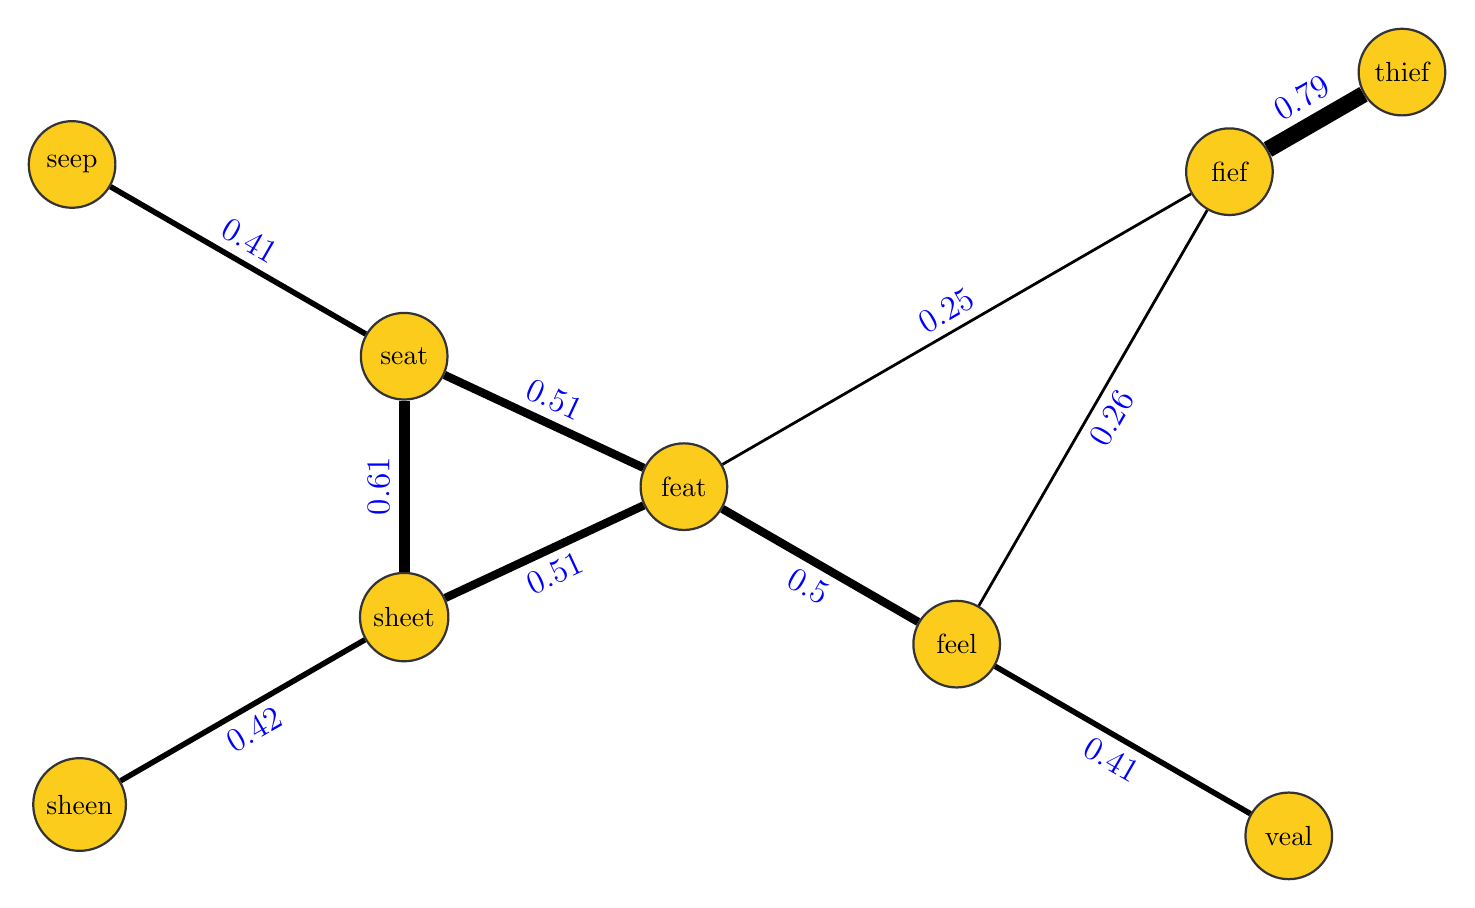
\begin{tikzpicture}[semithick]

% center 'ego' node at origin
\node[o] (feat) at (0,0) {feat};  

% add further nodes using polar notation [++(angle:radius)] relative
% to center node
\path (feat) ++(30:8) node (fief) [o] {fief};
\path (feat) ++(-30:4) node (feel) [o] {feel};
\path (feel) ++(-30:4.87) node (veal) [o] {veal};
\path (fief) ++(30:2.53) node (thief) [o] {thief};
\path (feat) ++(155:3.92) node (seat) [o] {seat};
\path (feat) ++(-155:3.92) node (sheet) [o] {sheet};
\path (sheet) ++(-150:4.76) node (sheen) [o] {sheen};
\path (seat) ++(150:4.87) node (seep) [o] {seep};

% add edges between nodes with text and line width indicating weights
\draw[line width=3] (feat) edge node[above, rotate=-25]{\large\color{blue} 0.51} (seat);
\draw[line width=3] (feat) edge node[below, rotate=25]{\large\color{blue} 0.51} (sheet);
\draw[line width=1] (feat) edge node[above, rotate=30]{\large\color{blue} 0.25} (fief);
\draw[line width=3] (feat) edge node[below, rotate=-30]{\large\color{blue} 0.5} (feel);
\draw[line width=4] (seat) edge node[above, rotate=90]{\large\color{blue} 0.61} (sheet);
\draw[line width=6] (thief) edge node[above, rotate=30]{\large\color{blue} 0.79} (fief);
\draw[line width=2] (feel) edge node[below, rotate=-30]{\large\color{blue} 0.41} (veal);
\draw[line width=2] (sheet) edge node[below, rotate=30]{\large\color{blue}  0.42} (sheen);
\draw[line width=2] (seat) edge node[above, rotate=-30]{\large\color{blue}  0.41} (seep);
\draw[line width=1] (feel) edge node[below, rotate=60]{\large\color{blue}  0.26} (fief);

\end{tikzpicture}


\end{document}
